\documentclass[conference]{IEEEtran}
\IEEEoverridecommandlockouts
\pdfoutput=1
% The preceding line is only needed to identify funding in the first footnote. If that is unneeded, please comment it out.
\usepackage{cite}
\usepackage{amsmath,amssymb,amsfonts, amsthm}
\usepackage{algorithmic}
\usepackage{graphicx}
\usepackage{textcomp}
\usepackage{xcolor}
\usepackage[shortlabels]{enumitem}
\usepackage{fancyhdr}
\usepackage{tikz}
\usepackage{lipsum}
\usepackage{hyperref}
\usepackage{wrapfig}
\usepackage{parskip}
\usepackage[a4paper, left=1in, right=1in, bottom=1in, top=0.5in]{geometry}
\usepackage{multirow}
\usepackage{gensymb}
\usepackage{placeins}
\usepackage{parindent}
\renewcommand{\figurename}{Gambar}
\renewcommand{\tablename}{TABEL}
\usetikzlibrary{shapes.geometric, arrows}
\usetikzlibrary {arrows.meta}
\usetikzlibrary{positioning}
\tikzstyle{node} = [rectangle, rounded corners, minimum width=7cm, text width=7cm, minimum height=1cm,text centered, draw=black]
\tikzstyle{arrow} = [ultra thick, line width=1.75mm, -{Triangle}, gray,fill=gray]
\def\BibTeX{{\rm B\kern-.05em{\sc i\kern-.025em b}\kern-.08em
    T\kern-.1667em\lower.7ex\hbox{E}\kern-.125emX}}


\pagestyle{fancy}
\fancyhf{} 
\renewcommand{\headrulewidth}{0pt}
\rfoot{\thepage}
\pagenumbering{arabic}



<<<<<<< HEAD
=======

>>>>>>> a0468ef39d3d0bcfeb7822e17a12a34c3b67d5fc
\makeatletter
\long\def\@makecaption#1#2{\ifx\@captype\@IEEEtablestring%
\footnotesize\begin{center}{\normalfont\footnotesize #1}\\
{\normalfont\footnotesize\scshape #2}\end{center}%
\@IEEEtablecaptionsepspace
\else
\@IEEEfigurecaptionsepspace
\setbox\@tempboxa\hbox{\normalfont\footnotesize {#1.}~~ #2}%
\ifdim \wd\@tempboxa >\hsize%
\setbox\@tempboxa\hbox{\normalfont\footnotesize {#1.}~~ }%
\parbox[t]{\hsize}{\normalfont\footnotesize \noindent\unhbox\@tempboxa#2}%
\else
\hbox to\hsize{\normalfont\footnotesize\box\@tempboxa\hfil}\fi\fi}
\makeatother

<<<<<<< HEAD
% Edit here
=======
>>>>>>> a0468ef39d3d0bcfeb7822e17a12a34c3b67d5fc

\begin{document}
\title{Judul Praktikum dengan \emph{Bahasa Asing}}


\author{\IEEEauthorblockN{\textbf{Nama Praktikan} (181xxxx)}
\IEEEauthorblockN{Kelompok X/ Hari, 1 Januari 2023}
\IEEEauthorblockN{Teknik Telekomunikasi}
\IEEEauthorblockN{Sekolah Teknik Elektro dan Informatika}
\IEEEauthorblockN{181190XX@telecom.stei.itb.ac.id}
\IEEEauthorblockN{Asisten: Nama Asisten}}

\maketitle
\thispagestyle{fancy}
\setlength{\parskip}{12pt}
\setlength{\parindent}{12pt}

\begin{abstract}
Bagian ini diisi oleh abstract. Menjelaskan tentang kegiatan praktikum yang dilakukan serta menjelaskan hasilnya. Sebagai contoh lihat abstrak berikut. Praktikum XXXX Modul X: Pengukuran resistansi pada rangkaian resistor sederhana memiliki tujuan untuk mengetahui cara menghitung parameter pada rangkaian resistor sederhana. Hasil yang ingin dicapai adalah mengetahui besaran resistansi, arus, dan voltase pada rangkaian resistor sederhana. Pada praktikum ini didapat hasil pengukuran yang sesuai dengan teori sehingga praktikum dinyatakan berhasil. Pada praktikum didapat hasil pengukuran yang tidak sesuai dengan teori, hal ini dikarenakan {sebutkan alasan mengapa hasil tidak sesuai}. Bentuk abstrak bisa beragam namun ditekankan bahwa abstrak harus mencakup semua isi dari laporan 
\end{abstract}

\begin{IEEEkeywords}
resistansi, resistor, [kata lain yang paling menggambarkan praktikum ini; format selalu menggunakan Italic]
\end{IEEEkeywords}

\setlength{\parskip}{6pt}
\setlength{\parindent}{12pt}

\section{Pendahuluan}
Pendahuluan adalah bagian laporan praktikum yang berisi penjelasan singkat tentang praktikum itu sendiri yang biasanya dimulai dari landasan teori yang singkat, pengertian – pengertian, dan alasan mengapa perlu dilakukan prakitikum ini. Lihat contoh pendahuluan berikut.

Resistor adalah sebuah komponen elektronik yang berguna untuk mengatur arus listrik yang mengalir pada sebuah rangkaian. Resistor dalam rangkaian memiliki tingkah laku yaitu mendisipasikan daya. Resistor banyak digunakan dalam devais elektronik seperti dalam computer, VNA, dll.

Maka dinilai perlu adanya kegiatan praktikum untuk memahami cara menghitung besaran pada rangkaian resistor, penulis telah melakukan praktikum {Judul Praktikum dengan Bahasa Asing} yang memiliki tujuan sebagai berikut:

\begin{enumerate}[1., leftmargin=1cm]
    \item Tujuan praktikum 1
    \item Tujuan Praktikum 2
\end{enumerate}

\section{Dasar Teori}

\subsection{Resistor}

Resistor adalah komponen elektronik yang mendisipasikan daya [1]. Angka 1 di samping digunain sebagai reference. Setiap yang ada pada dasar teori harus mengambil pada sumber yang kredibel seperti buku, jurnal, paper, atau web yang kredibel. Setiap kali mengutip dari sumber jangan lupa beri reference angka. Tiap angka nanti akan disitasi kembali pada bagian ke-6 laporan praktikum yaitu daftar pustaka. Dasar teori juga biasanya menampilkan gambar, untuk format penulisan lihat gambar berikut

\begin{figure}[htbp]
\centerline{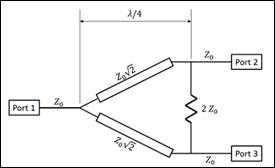
\includegraphics{./Figures/two-way.png}}
\caption{Rangkaian Two-Way Wilkinson Power Divider [1].}
\label{fig1}
\end{figure}
\FloatBarrier

Dalam dasar teori juga dapat menampilkan formula atau persamaan yang digunakan dalam analisis. Persamaan yang digunakan penulisannya sebagai berikut.

\begin{equation}
    V = I.R
\end{equation}

Pada persamaan di atas, lihat angka (1) pada bagian samping. Angka tersebut digunakan ketika ingin merefer formula terkait pada baigan analisis. Sebagai contoh, pada analisis tidak ditulis “dengan menggunakan rumus V = IR, didapat tegangan sebesar …” namun ditulis “dengan menggunakan rumus/persamaan (1) didapat tegangan sebesar …” tentu ini dapat disesuaikan sesuai kondisi laporan. Misal pada analisis perlu penjelasan tahap per tahap dalam menghitung nilai akhir demi penjelasan yang lebih rinci, maka penulisan perhitungan tahap per tahap menggunakan rumus di atas tetap diperlukan.

\subsection{Sub Teori Kedua}

Dasar teori tidak boleh copas dari modul praktikum namun menjadikan modul praktikum sebagai sumber dan disitasi diperbolehkan. Tanyakan ke asisten masing – masing tentang hal ini karena praktikum berbeda kadang memiliki kondisi yang berbeda.

\section{Metodologi Percobaan}

\subsection{Alat Percobaan}
\begin{enumerate}[1., leftmargin=1cm]
    \item Alat Percobaan 1
    \item Alat Percobaan 2
    \item dst [cantumkan semua alat percobaan lainnya yang digunakan dalam praktikum] 
\end{enumerate}

\subsection{Langkah Kerja}
Langkah-langkah percobaan pada Modul X : Judul Praktikum dengan \textit{Bahasa Asing} adalah sebagai berikut.

\subsubsection{Percobaan 1: Kalibrasi Alat Ukur}\hfill
\begin{center}
    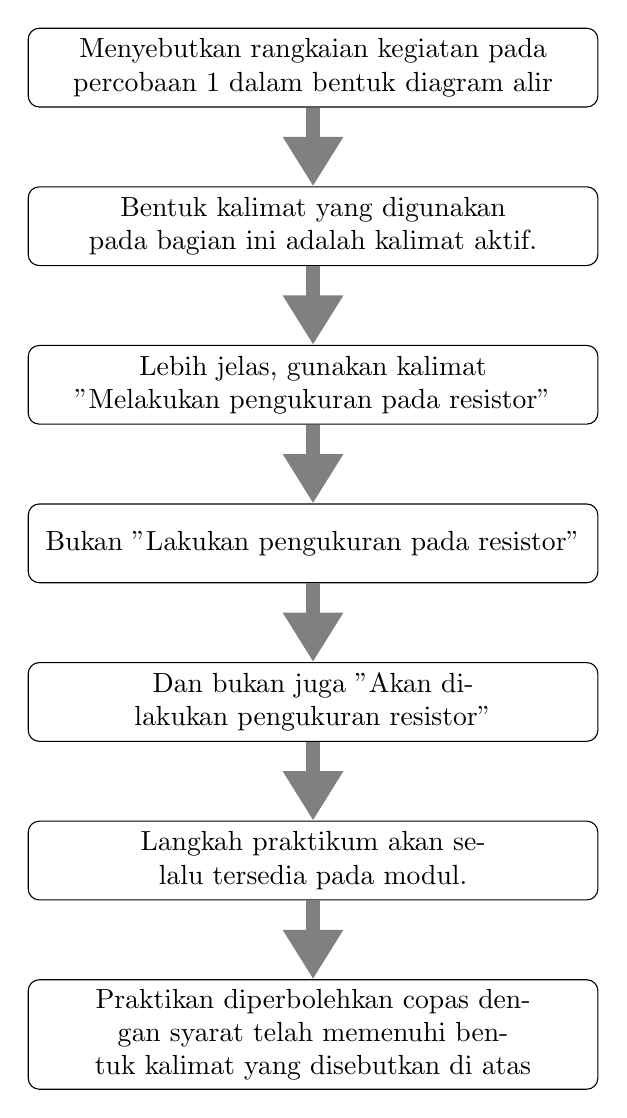
\begin{tikzpicture}[node distance=1cm, auto]
    \node (p11) [node] {Menyebutkan rangkaian kegiatan pada percobaan 1 dalam bentuk diagram alir
};
    \node (p12) [node, below = of p11] {Bentuk kalimat yang digunakan pada bagian ini adalah kalimat aktif. 
};
    \node (p13) [node, below = of p12] {Lebih jelas, gunakan kalimat "Melakukan pengukuran pada resistor"
};
    \node (p14) [node, below = of p13] {Bukan "Lakukan pengukuran pada resistor"
};
    \node (p15) [node, below = of p14] {Dan bukan juga "Akan dilakukan pengukuran resistor"
};
    \node (p16) [node, below = of p15] {Langkah praktikum akan selalu tersedia pada modul. 
};
    \node (p17) [node, below = of p16] {Praktikan diperbolehkan copas dengan syarat telah memenuhi bentuk kalimat yang disebutkan di atas 
};
    \draw [arrow] (p11) -- (p12);
    \draw [arrow] (p12) -- (p13);
    \draw [arrow] (p13) -- (p14);
    \draw [arrow] (p14) -- (p15);
    \draw [arrow] (p15) -- (p16);
    \draw [arrow] (p16) -- (p17);
    \end{tikzpicture}
\end{center}

\subsubsection{Percobaan 2: ...}\hfill
\begin{center}
    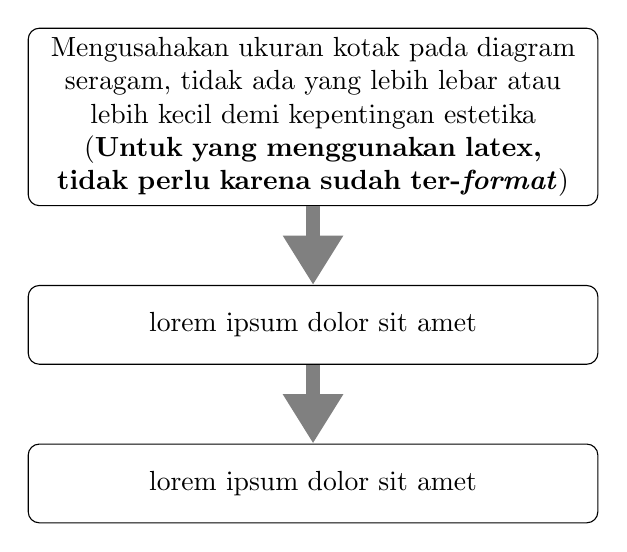
\begin{tikzpicture}[node distance=1cm]
    \node (p21) [node] {Mengusahakan ukuran kotak pada diagram seragam, tidak ada yang lebih lebar atau lebih kecil demi kepentingan estetika (\textbf{Untuk yang menggunakan latex, tidak perlu karena sudah ter-\textit{format}})
};
    \node (p22) [node, below = of p21] {lorem ipsum dolor sit amet
};
    \node (p23) [node, below = of p22] {lorem ipsum dolor sit amet
};
    \draw [arrow] (p21) -- (p22);
    \draw [arrow] (p22) -- (p23);
    \end{tikzpicture}
\end{center}

\section{Hasil dan Analisis Percobaan}

\subsection{Percobaan 1: Kalibrasi Alat Ukur}

[Menjelaskan analisis percobaan, subjudul selalu menggunakan format \textit{Italic}].\\

Pada percobaan ini akan dilakukan kalibrasi alat ukur dengan menggunakan modul … . Pada bagian analisis, dijelaskan secara runtut langkah praktikum dari awal hingga akhir serta hasil data yang diperoleh pada setiap langkahnya (jika ada). Tidak seperti pada bagian langkah kerja, bentuk kalimat yang digunakan adalah kalimat pasif. Perhatikan contoh berikut. Pada hasil dan analisis gunakan kalimat seperti “Kemudian akan diukur tegangan antara titik A dan B dengan menggunakan voltmeter. Data pengukuran disajikan pada tabel berikut”. Hindari penggunaan kalimat aktif seperti “mengukur voltase antara titik A dan B dengan menggunakan voltmeter sehingga memperoleh data sebagai berikut”.

\begin{figure}[htbp]
\centerline{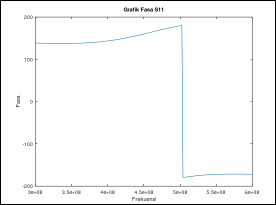
\includegraphics{./Figures/s11.png}}
\caption{Grafik Fasa S11}
\label{fig2}
\end{figure}
\FloatBarrier

Selalu beri penjelasan setelah gambar dan jangan biarkan gambar ditampilkan tanpa penjelasan setelahnya. Contoh nya seperti berikut “Gambar \ref{fig2} menunjukkan grafik fasa S11 …”

\subsection{Percobaan 2:...}
Apabila terdapat tabel data, maka gunakan format berikut

\begin{table}[htbp]
\caption{Hasil Pengukuran ...}
\begin{center}
\begin{tabular}{|c|c|c|}
\hline
\multicolumn{3}{|c|}{\textbf{Table Column Head}} \\
\cline{1-3} 
\textbf{\textit{Table column subhead}}& \textbf{\textit{Subhead}}& \textbf{\textit{Subhead}} \\
\hline
 More table copy & lorem & ipsum  \\
\hline
\end{tabular}
\label{tab1}
\end{center}
\end{table}

Dalam merujuk tabel gunakan contoh sebagai berikut. “Tabel \ref{tab1} menunjukkan hasil pengamatan osilator collpits osilasi maksimum ketika switch N”.

Poin penting pada analisis selain menjelaskan kegiatan praktikum tiap tahapnya adalah membandingkan hasil yang didapat secara percobaan dengan teori yang ada. Ada beberapa kemungkinan yang akan terjadi yaitu hasil sesuai teori dan tidak sesuai. Jelaskan bahwa hasil telah sesuai teori jika sudah sesuai, dan jelaskan bahwa hasil tidak sesuai teori jika tidak. Apabila tidak sesuai teori, jelaskan juga alasannya mengapa hal tersebut bisa terjadi. Kemungkinan lainnya adalah hasil secara percobaan sedikit melenceng dari nilai teori sehingga bisa dijelaskan kenapa seperti itu, misalnya karena kesalahan pengukuran atau pengaruh lingkungan dsb. Asumsikan juga alat praktikum telah dikalibrasi dan sedang dalam kondisi baik sehingga tidak diperbolehkan menyalahkan alat praktikum.

\section{Kesimpulan}
Kesimpulan berisi tentang kesimpulan laporan praktikum. Bentuknya adalah per paragraf dan tiap paragraf menjawab tiap poin pada tujuan praktikum. Jika praktikum mempunyai 3 poin tujuan, maka 3 poin tersebut dijelaskan pada 3 paragraf kesimpulan. Karena kesimpulan memastikan seluruh kegiatan praktikum disampaikan, maka perlu dilihat ulang apakah tujuan praktikum kalian melingkupi seluruh kegiatan praktikum.

Panduan penulisan lengkap template paper IEEE A4 dalam format docx dapat dilihat pada link berikut. \url{https://www.ieee.org/conferences/publishing/templates.html}.

% Jika tidak menggunakan bibtex, uncomment code di bawah ini
%
\begin{thebibliography}{00}
\bibitem{b1} G. Eason, B. Noble, and I. N. Sneddon, ``On certain integrals of Lipschitz-Hankel type involving products of Bessel functions,'' Phil. Trans. Roy. Soc. London, vol. A247, pp. 529--551, April 1955.
\bibitem{b2} J. Clerk Maxwell, A Treatise on Electricity and Magnetism, 3rd ed., vol. 2. Oxford: Clarendon, 1892, pp.68--73.
\bibitem{b3} I. S. Jacobs and C. P. Bean, ``Fine particles, thin films and exchange anisotropy,'' in Magnetism, vol. III, G. T. Rado and H. Suhl, Eds. New York: Academic, 1963, pp. 271--350.
\bibitem{b4} K. Elissa, ``Title of paper if known,'' unpublished.
\bibitem{b5} R. Nicole, ``Title of paper with only first word capitalized,'' J. Name Stand. Abbrev., in press.
\bibitem{b6} Y. Yorozu, M. Hirano, K. Oka, and Y. Tagawa, ``Electron spectroscopy studies on magneto-optical media and plastic substrate interface,'' IEEE Transl. J. Magn. Japan, vol. 2, pp. 740--741, August 1987 [Digests 9th Annual Conf. Magnetics Japan, p. 301, 1982].
\bibitem{b7} M. Young, The Technical Writer's Handbook. Mill Valley, CA: University Science, 1989.
\end{thebibliography}

%% Jika ingin menggunakan bibtex, silakan uncomment code di bawah ini

%\bibliographystyle{plain}
%\bibliography{refs}


\section*{Biografi Singkat}

\begin{wrapfigure}{l}{0.15\textwidth} %this figure will be at the left
    \centering
    
\includegraphics[width=0.15\textwidth]{./Figures/pas-foto.png}
\end{wrapfigure}

\noindent Berikan biografi singkat kalian dalam ini. Biografi yang ditulis diharapkan biografi serius. Lorem ipsum dolor sit amet, consectetur adipiscing elit, sed do eiusmod tempor incididunt ut labore et dolore magna aliqua. Ut enim ad minim veniam, quis nostrud exercitation ullamco laboris nisi ut aliquip ex ea commodo consequat. Duis aute irure dolor in reprehenderit in voluptate velit esse cillum dolore eu fugiat nulla pariatur. Excepteur sint occaecat cupidatat non proident, sunt in culpa qui officia deserunt mollit anim id est laborum


\end{document}
